\section{Preliminary}
Before introducing ReSum, we review the ReAct paradigm to provide necessary background and highlight the fundamental challenges that motivate our research.

ReAct~\citep{yao2023react} is a widely adopted agentic workflow~\citep{li2025websailor, wu2025webdancer, li2025search} where agents perform iterative cycles of Thought, Action, and Observation. Specifically, in each iteration, the LLM generates a reasoning step (Thought) based on existing context, emits a parsable tool call (Action), and receives feedback from the environment (Observation). In web search contexts, the action space typically consists of search queries, webpage browsing, or generating the final answer. The iteration terminates when the agent produces a final answer. A complete trajectory with $T$ iterations can be formally defined as:
\[
\mathcal{H}_T = \big(q, \tau_1, a_1, o_1, \ldots, \tau_{T-1}, a_{T-1}, o_{T-1}, \tau_T, a_T\big),
\]
where $q$ is the question, and $\tau_i$, $a_i$, and $o_i$ represent the thought, action, and observation at the $i$-th round, respectively. At step $t$, both the thought $\tau_t$ and action $a_t$ are sampled from a policy model $\pi_{\theta}$ conditioned on all previous context as $(\tau_t, a_t) \sim \pi_{\theta}(\cdot \mid \mathcal{H}_{t-1})$.

For complex web search tasks with highly ambiguous entities and relationships, agents must perform extensive tool interactions to gather disparate evidence and converge on a solution. However, continuously appending the full interaction history quickly exhausts modern LLMs’ context windows before difficult cases can be resolved. To illustrate this limitation, we analyze the behavior of WebSailor-7B~\citep{li2025websailor} on the challenging BrowseComp benchmark~\citep{bc_en}. As shown in Figure~\ref{fig:token_comp}, while solved cases generally fit within the context window, failed trajectories frequently exceed the 32$k$ limit, necessitating truncation.

\begin{figure}[!t]
    \centering
    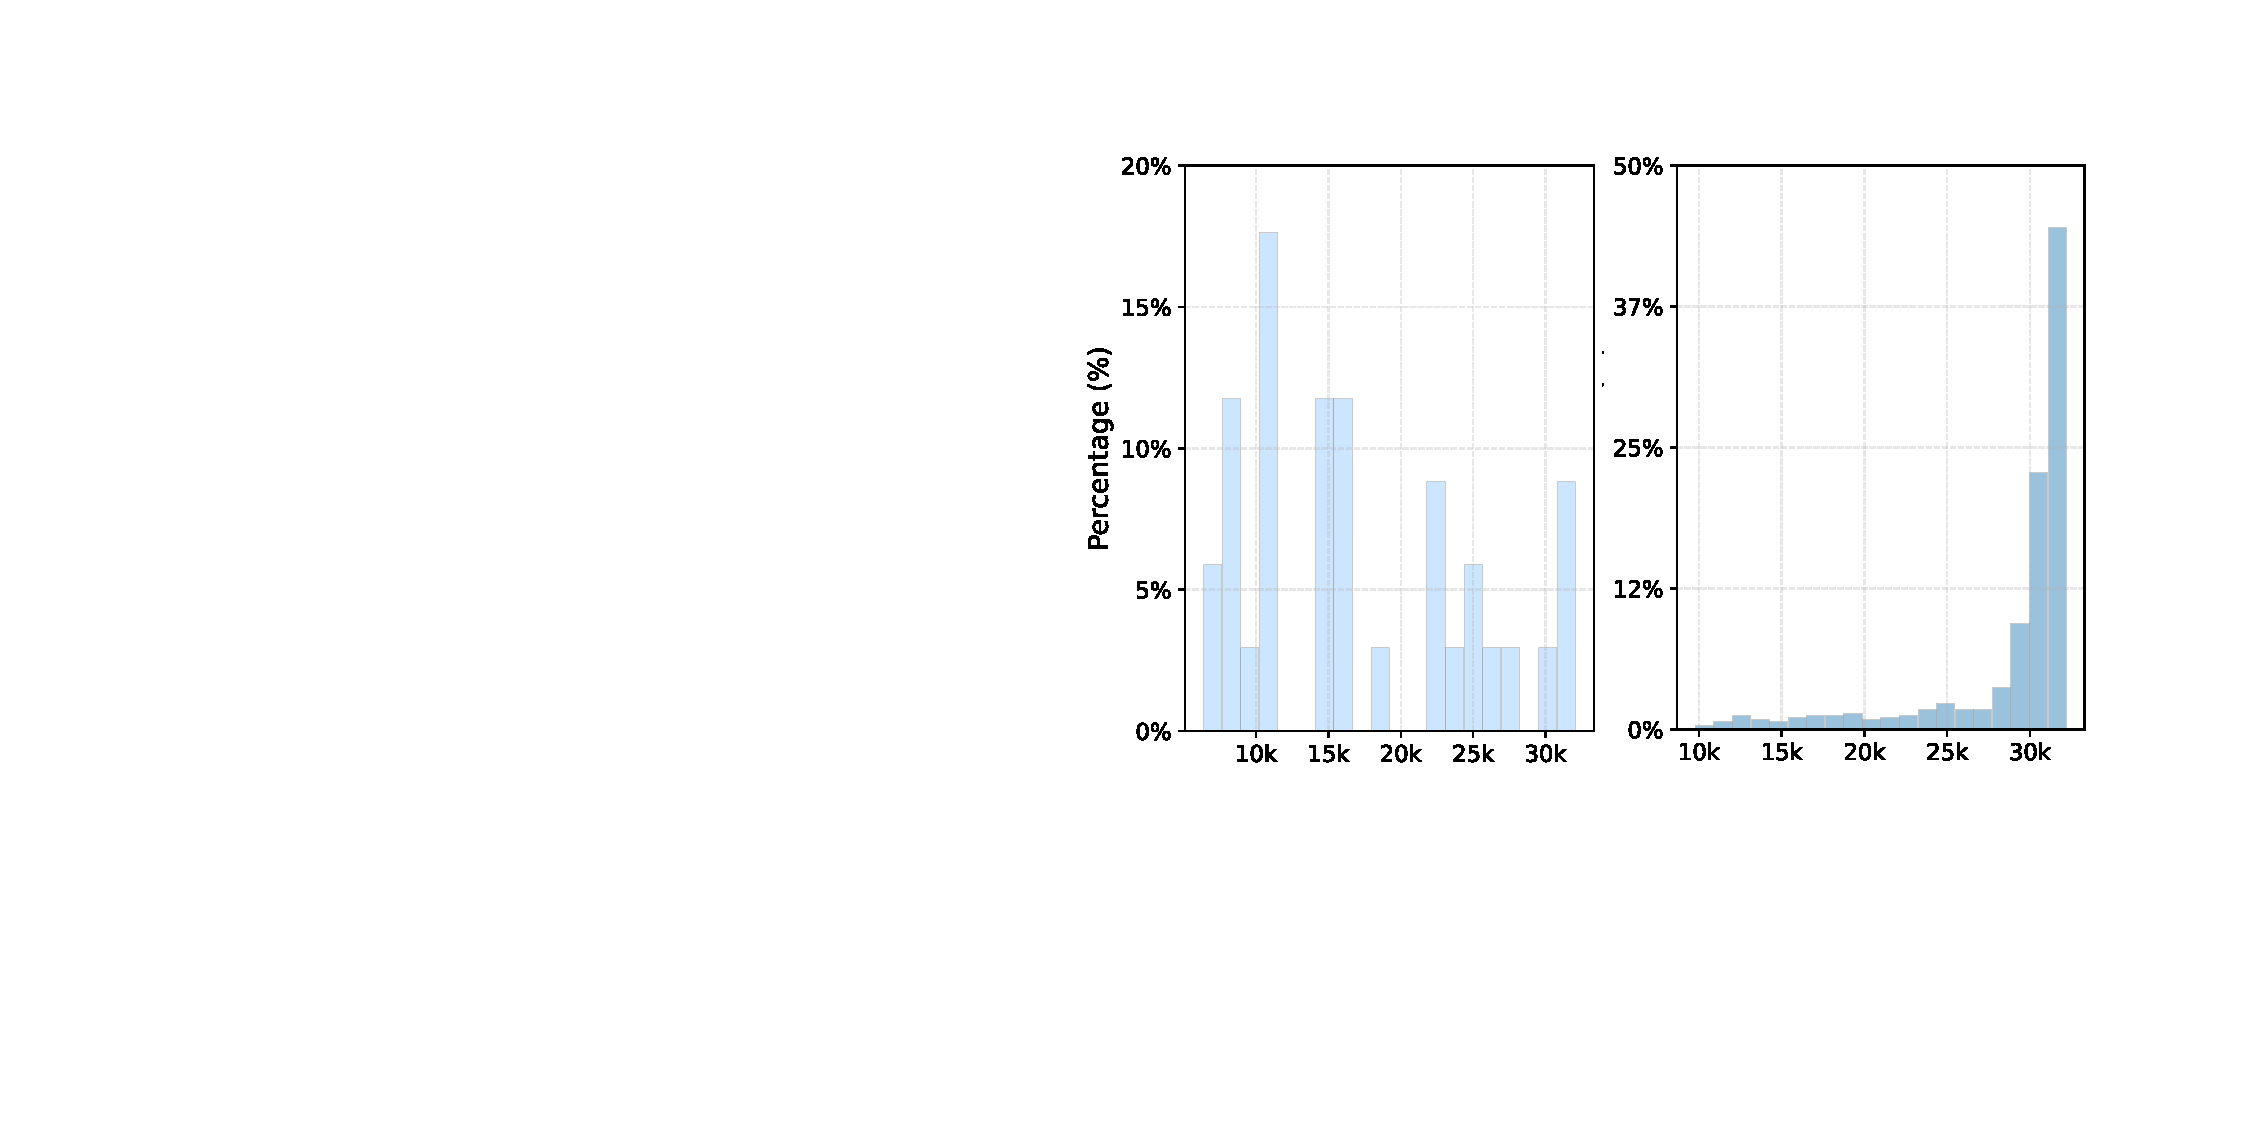
\includegraphics[width=0.46\textwidth]{images/token_comp_percentage.pdf}
    \caption{\textbf{Context limits in ReAct constrain exploration.} We compare token consumption distributions for \textcolor[HTML]{8EC7FF}{\textbf{correct}} (left) and \textcolor[HTML]{1F77B4}{\textbf{incorrect}} (right) samples using WebSailor‑7B~\citep{li2025websailor} on BrowseComp~\citep{bc_en}. Failed cases consume significantly more tokens, indicating that trajectories are frequently truncated before resolution.}
    \label{fig:token_comp}
    \vspace*{-10pt}
\end{figure}

Following existing web agent designs~\citep{li2025websailor, gao2025asearcher, li2025chainofagent}, we implement two essential tools for web exploration: \texttt{Search} queries the Google Search engine, accepting multiple queries simultaneously and returning the top-10 results per query, and \texttt{Visit} browses specific web pages by URL using Jina~\citep{jina} and extracts goal-specific evidence using Qwen2.5-72B-Instruct~\citep{qwen2.5}. The discussion of existing research on web agents and context management for agents has been moved to \textbf{Appendix~\ref{appendix:related_work}}.
